\documentclass[lmodern, utf8, diplomski, numeric]{fer}
\usepackage{booktabs}

\begin{document}

% TODO: Navedite broj rada.
\thesisnumber{1115}

% TODO: Navedite naslov rada.
\title{DUBOKE KONVOLUCIJSKE NEURONSKE MREŽE ZA RASPOZNAVANJE ZNAKOVA}

% TODO: Navedite vaše ime i prezime.
\author{Matija Ilijaš}

\maketitle

% Ispis stranice s napomenom o umetanju izvornika rada. Uklonite naredbu \izvornik ako želite izbaciti tu stranicu.

% Dodavanje zahvale ili prazne stranice. Ako ne želite dodati zahvalu, naredbu ostavite radi prazne stranice.
\zahvala{}

\tableofcontents

\chapter{Uvod}
Uvod rada. Nakon uvoda dolaze poglavlja u kojima se obrađuje tema.

\chapter{Optičko prepoznavanje znakova}

\chapter{Umjetne neuronske mreže}

Umjetna neuronska mreža je algoritam strojnog učenja inspiriran strukturom i funkcionalnošću ljudskog mozga. Zasniva se na paralelnoj obradi podataka, te vrlo dobro rješava sve probleme kod kojih postoji složena nelinearna veza ulaza i izlaza. Radi s velikim brojem parametara i varijabli, te može raditi s nejasnim podacima što ju čini robusnom na pogreške. Zbog svoje robusnosti, najčešća primjena neuronske mreže je u raspoznavanju uzoraka, obradi slike i govora, nelinearnom upravljanju itd.

Mreža se sastoji od tri vrste sloja: ulaznog, izlaznog, te skrivenog koji povezuje prethodna dva. Čvorišta, tzv. neuroni, skrivenog sloja povezani su težinskim vezama s ulaznim i izlaznim neuronima. Dvije su faze rada umjetnih neuronskih mreža: učenje (treniranje) i obrada podataka (eksploatacija). Učenje je iterativan postupak predočavanja ulaznih primjera i očekivanog izlaza pri čemu dolazi do postupnog prilagođavanja težina veza neurona. Nakon što se težine skrivenog sloja prilagode postupkom treniranja, eksploatacijom neuronske mreže može se za do tad neviđeni ulazni primjer dobiti pripadajući izlaz.


\chapter{Duboke konvolucijske neuronske mreže}

\chapter{Implementacija}

U sklopu ovog rada razvijen je sustav za učenje i testiranje različitih arhitektura neuronskih mreža. Prilikom razvijanja takvog sustava bilo je važno zadovoljiti dva glavna uvjeta: brzo učenje novih arhitektura na velikoj količini podataka te detaljna analiza rada naučenih mreža. Iz tog razloga sustav je podijeljen na dva podsustava razvijena sa zasebnim alatima. Podsustav zadužen za učenje implementiran je u razvojnom alatu Torch koji omogućuje paralelno izvođenje procesa učenja na grafičkoj kartici. Podsustav koji provodi analizu rada naučenih mreža implementiran je u jeziku C++ korištenjem OpenCV biblioteke.

\section{Sustav za učenje}

Kako bi cijeli proces istraživanja različitih arhitektura mreža i podataka bio što efikasniji, potrebno je prije svega imati brzi sustav za učenje. Učenje velikih arhitektura na velikoj količini podataka može trajati tjednima, pa i mjesecima, sekvencijalnim računanjem na standarnom procesoru računala. Stoga je tek pojavom kvalitetnih biblioteka, koje omogućuju optimizirano paralelno računanje na grafičkoj kartici, postalo moguće provoditi istraživanje u području dubokog učenja. 
Osim brzine učenja, važna je i jednostavnost definiranja parametara mreže koja se uči, kao i parametara samog procesa učenja. Kod implementacije ovog rada odabran je razvojni alat Torch zbog svoje jednostavnosti i brzine, ali i podrške velikih kompanija kao što su Facebook i Google, koje nerijetko dijele korisne implementacije sa zajednicom. 

\subsection{Torch razvojni alat}

Prilikom odabira razvojnog alata uzeti su u obzir i alati Caffe i Theano. Možda najpopularniji alat za duboko učenje Caffe ima izrazito jednostavno sučelje za odabir parametara mreže i procesa učenja, no kao posljedica toga teško je raditi promjene u postojećoj implementaciji u svrhu istraživanja ili razvoja. Theano s druge strane pruža puno manju razinu apstrakcije te ostavlja mogućnost lake izmjene većine implementacije, no postaje nepraktičan kod česte upotrebe standarnih algoritama.
Torch je po razini apstrakcije negdje između prethodno navedenih alata, dovoljno je niske apstrakcije za laku izmjenu implementacije kod razvoja i istraživanja, ali ima i sučelje za standarne algoritme koje ga čini praktičnim. 

Brzina samog izvođenja procesa učenja na grafičkim karticama velikim dijelom ovisi o pozadinskoj implementaciji paralelnog računanja koja je za sve navedene alate otprilike podjednako brza, te se toliko često mijenja da nema smisla uspoređivati njihove brzine. S druge strane, važan faktor kod odabira alata je podrška akademske zajednice i industrije s obzirom da o tome ovisi koliko brzo se razvijaju implementacije novih koncepata. Torch ima implementaciju za većinu novih koncepata u dubokom učenju zbog podrške kompanija kao što su Google, Facebook i Twitter.  Tako je primjerice implementirana relativno nova metoda Dropout za regularizaciju prilikom učenja mreže te ReLU funkcija prijelaza koja je pokazale bolje rezultate od standardne sigmoidalne funkcije u nedavnim istraživanjima.

Sama implementacija Torcha podijeljena je na dva dijela. Sve računske operacije na grafičkoj kartici napisane su kao C/CUDA implementacija za maksimalnu brzinu, dok je ostatak funkcionalnosti implementiran u skriptnom jeziku LuaJIT za lakše korištenje alata.  

\subsection{Definiranje arhitekture}
	
Neuronska mreža je u Torch alatu definirana kao model koji se sastoji od sekvencijalno povezanih slojeva koji vrše različite računske operacije.
Tako bi na primjer jedna standarna neuronska mreža s jednim skrivenim slojem bila definirana kao sekvencijalni niz prikazan na Slici ???. 

\begin{figure}[ht!]
\centering
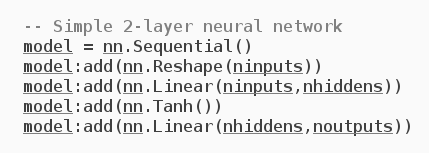
\includegraphics[width=9cm]{slike/nn_model.png}
\caption{}
\end{figure}

Primjer jedne duboke konvolucijske mreže definirane kao Torch model prikazan je na Slici ???.

\begin{figure}[ht!]
\centering
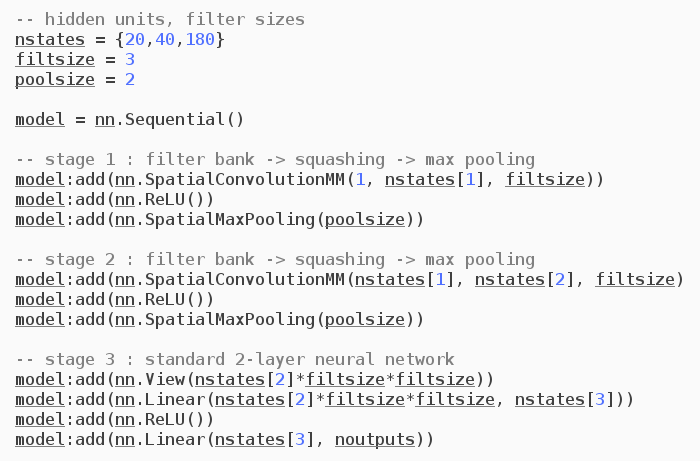
\includegraphics[width=16cm]{slike/cnn_model.png}
\caption{}
\end{figure}

\subsection{Definiranje parametara učenja}



\section{Sustav za testiranje}

\chapter{Rezultati}

\chapter{Zaključak}
Zaključak.

\bibliography{literatura}
\bibliographystyle{fer}

\begin{sazetak}


\kljucnerijeci{Ključne riječi, odvojene zarezima.}
\end{sazetak}

% TODO: Navedite naslov na engleskom jeziku.
\engtitle{Deep convolutional neural networks for character recognition}
\begin{abstract}
Abstract.

\keywords{Keywords.}
\end{abstract}

\end{document}
